% This is "sig-alternate.tex" V2.1 April 2013
% This file should be compiled with V2.8 of "sig-alternate.cls" May 2012
%
% This example file demonstrates the use of the 'sig-alternate.cls'
% V2.8 LaTeX2e document class file. It is for those submitting
% articles to ACM Conference Proceedings WHO DO NOT WISH TO
% STRICTLY ADHERE TO THE SIGS (PUBS-BOARD-ENDORSED) STYLE.
% The 'sig-alternate.cls' file will produce a similar-looking,
% albeit, 'tighter' paper resulting in, invariably, fewer pages.
%
% ----------------------------------------------------------------------------------------------------------------
% This .tex file (and associated .cls V2.8) produces:
%       1) The Permission Statement
%       2) The Conference (location) Info information
%       3) The Copyright Line with ACM data
%       4) NO page numbers
%
% as against the acm_proc_article-sp.cls file which
% DOES NOT produce 1) thru' 3) above.
%
% Using 'sig-alternate.cls' you have control, however, from within
% the source .tex file, over both the CopyrightYear
% (defaulted to 200X) and the ACM Copyright Data
% (defaulted to X-XXXXX-XX-X/XX/XX).
% e.g.
% \CopyrightYear{2007} will cause 2007 to appear in the copyright line.
% \crdata{0-12345-67-8/90/12} will cause 0-12345-67-8/90/12 to appear in the copyright line.
%
% ---------------------------------------------------------------------------------------------------------------
% This .tex source is an example which *does* use
% the .bib file (from which the .bbl file % is produced).
% REMEMBER HOWEVER: After having produced the .bbl file,
% and prior to final submission, you *NEED* to 'insert'
% your .bbl file into your source .tex file so as to provide
% ONE 'self-contained' source file.
%
% ================= IF YOU HAVE QUESTIONS =======================
% Questions regarding the SIGS styles, SIGS policies and
% procedures, Conferences etc. should be sent to
% Adrienne Griscti (griscti@acm.org)
%
% Technical questions _only_ to
% Gerald Murray (murray@hq.acm.org)
% ===============================================================
%
% For tracking purposes - this is V2.0 - May 2012

\documentclass{sig-alternate}



\begin{document}

% Copyright
\setcopyright{waclicense}


%% DOI
%\doi{10.475/123_4}
%
%% ISBN
%\isbn{123-4567-24-567/08/06}
%
%%Conference
%\conferenceinfo{PLDI '13}{June 16--19, 2013, Seattle, WA, USA}
%
%\acmPrice{\$15.00}

%
% --- Author Metadata here ---
\conferenceinfo{Web Audio Conference WAC-2016,}{April 4--6, 2016, Atlanta, USA}
\CopyrightYear{2016} % Allows default copyright year (20XX) to be over-ridden - IF NEED BE.
%\crdata{0-12345-67-8/90/01}  % Allows default copyright data (0-89791-88-6/97/05) to be over-ridden - IF NEED BE.
% --- End of Author Metadata ---

\title{BPMTimeline: JavaScript Tempo Functions and Time Mappings using an Analytical Solution}
%\subtitle{[Extended Abstract]
%\titlenote{A full version of this paper is available as
%\textit{Author's Guide to Preparing ACM SIG Proceedings Using
%\LaTeX$2_\epsilon$\ and BibTeX} at
%\texttt{www.acm.org/eaddress.htm}}}
%
% You need the command \numberofauthors to handle the 'placement
% and alignment' of the authors beneath the title.
%
% For aesthetic reasons, we recommend 'three authors at a time'
% i.e. three 'name/affiliation blocks' be placed beneath the title.
%
% NOTE: You are NOT restricted in how many 'rows' of
% "name/affiliations" may appear. We just ask that you restrict
% the number of 'columns' to three.
%
% Because of the available 'opening page real-estate'
% we ask you to refrain from putting more than six authors
% (two rows with three columns) beneath the article title.
% More than six makes the first-page appear very cluttered indeed.
%
% Use the \alignauthor commands to handle the names
% and affiliations for an 'aesthetic maximum' of six authors.
% Add names, affiliations, addresses for
% the seventh etc. author(s) as the argument for the
% \additionalauthors command.
% These 'additional authors' will be output/set for you
% without further effort on your part as the last section in
% the body of your article BEFORE References or any Appendices.

\numberofauthors{3} %  in this sample file, there are a *total*
% of EIGHT authors. SIX appear on the 'first-page' (for formatting
% reasons) and the remaining two appear in the \additionalauthors section.
%
\author{
% You can go ahead and credit any number of authors here,
% e.g. one 'row of three' or two rows (consisting of one row of three
% and a second row of one, two or three).
%
% The command \alignauthor (no curly braces needed) should
% precede each author name, affiliation/snail-mail address and
% e-mail address. Additionally, tag each line of
% affiliation/address with \affaddr, and tag the
% e-mail address with \email.
%
% 1st. author
\alignauthor
Bruno Dias\\
       \affaddr{INESC-ID, IST - Universidade de Lisboa}\\
       \email{bruno.s.dias@ist.utl.pt}
% 2nd. author
\alignauthor
David M. Matos\\
       \affaddr{INESC-ID, IST - Universidade de Lisboa}\\
       \email{david.matos@inesc-id.pt }
% 3rd. author
\alignauthor H. Sofia Pinto\\
       \affaddr{INESC-ID, IST - Universidade de Lisboa}\\
       \email{sofia@inesc-id.pt }
}
% There's nothing stopping you putting the seventh, eighth, etc.
% author on the opening page (as the 'third row') but we ask,
% for aesthetic reasons that you place these 'additional authors'
% in the \additional authors block, viz.
\date{1 September 2015}
% Just remember to make sure that the TOTAL number of authors
% is the number that will appear on the first page PLUS the
% number that will appear in the \additionalauthors section.

\maketitle
\begin{abstract}
Time mapping is a common feature in many (commercial and/or open-source) Digital Audio Workstations, allowing the musician to automate tempo changes of a musical performance or work, as well as to visualize the relation between score time (beats) and real/performance time (seconds). Unfortunately, available music production, performance and remixing tools implemented with web technologies like JavaScript and Web Audio API do not offer any mechanism for flexible, and seamless, tempo manipulation and automation.

In this paper, we present BPMTimeline, a time mapping library, providing a seamless mapping between score and performance time. To achieve this, we model tempo changes as tempo functions (a well documented subject in literature) and realize the mappings through integral and inverse of integral of tempo functions.
\end{abstract}


%
% The code below should be generated by the tool at
% http://dl.acm.org/ccs.cfm
% Please copy and paste the code instead of the example below. 
%
%\begin{CCSXML}
%<ccs2012>
 %<concept>
  %<concept_id>10010520.10010553.10010562</concept_id>
  %<concept_desc>Computer systems organization~Embedded systems</concept_desc>
  %<concept_significance>500</concept_significance>
 %</concept>
 %<concept>
  %<concept_id>10010520.10010575.10010755</concept_id>
  %<concept_desc>Computer systems organization~Redundancy</concept_desc>
  %<concept_significance>300</concept_significance>
 %</concept>
 %<concept>
  %<concept_id>10010520.10010553.10010554</concept_id>
  %<concept_desc>Computer systems organization~Robotics</concept_desc>
  %<concept_significance>100</concept_significance>
 %</concept>
 %<concept>
  %<concept_id>10003033.10003083.10003095</concept_id>
  %<concept_desc>Networks~Network reliability</concept_desc>
  %<concept_significance>100</concept_significance>
 %</concept>
%</ccs2012>  
%\end{CCSXML}
%
%\ccsdesc[500]{Computer systems organization~Embedded systems}
%\ccsdesc[300]{Computer systems organization~Redundancy}
%\ccsdesc{Computer systems organization~Robotics}
%\ccsdesc[100]{Networks~Network reliability}
%
%
%%
%% End generated code
%%
%
%%
%%  Use this command to print the description
%%
%\printccsdesc
%
%% We no longer use \terms command
%%\terms{Theory}
%
%\keywords{ACM proceedings, \LaTeX, text tagging}

\section{Introduction}

Tempo manipulation of a musical expression or works is used to (1) make a musical expression, or work, more lively (through a faster tempo) or more solemn (slower tempo); (2) allow a DJ to synchronize the tempo of several songs playing simultaneously,  to align the beats; (3) create climaxes in a musical expression or work. Mainstream Digital Audio Workstations (DAWs), either commercial and/or open-source, like Ableton Live, figure \ref{fig:abletonautomation}, Logic Pro and Reaper allow tempo automation through time maps, offering a seamless relation between performance and score time, using a tempo function. Unfortunately, to the best of our knowledge, there are no time mapping implementations in JavaScript. 

\begin{figure}
	%COLOCAR A IMAGEM ableton-tempo-automation.png [width=7in]
	\includegraphics[width=3.5in]{ableton-tempo-automation-1.png}
	\caption{Tempo automation example in Ableton Live, using step and linear tempo functions.}
	\label{fig:abletonautomation} 
\end{figure}

In this paper, we present the theory supporting time maps as well as our JavaScript implementation, BPMTimeline. The development of BPMTimeline followed three non-functional requirements:

\begin{itemize}
	\item \textbf{No real impact on application performance:} the temporal overhead for time mapping and tempo search should remain unnoticed;

	\item \textbf{Seamless tempo manipulation:} the developer should not be restricted to crisp tempo changes (e.g.: step functions) nor should tempo changes be only allowed on restricted time marks (e.g.: the beginning of a beat or measure);

	\item \textbf{Easy to integrate:} the implementation should be self-contained, with no need to include external libraries.
\end{itemize}

In section 3, we describe essential theoretical definitions regarding the relation between score and real time. In section 4, we detail our implementation. Finally, in section 5, we describe some use cases for BPMTimeline.

Our implementation and demo pages are currently hosted at GitHub.\footnote{https://github.com/echo66/bpm-timeline.js}


\section{Related Work}

Time mapping is a well document subject \cite{Dannenberg:1997,Kirke:2009,honing:time2time,wheresthebeat,honing:1993}. The main idea of a time map is to relate score time (beats) with real/performance time (seconds) through mathematical manipulation of  tempo functions. A tempo function \textit{T} maps score, or performance, time to a tempo value, e.g.: $T(63\,secs) = 105.12\,bpm$). Besides tempo functions and time maps, another way of representing expressive tempo manipulation and timing is through time shifts \cite{honing:time2time}, a function that expresses deviations of certain events in relation to a reference score/performance time line.

Available JavaScript live coding frameworks and DAWs do not offer time maps. In frameworks like Flocking \cite{flocking:icmc2014}, tempo manipulation is achieved through manual and crisp changes, and tempo automation can be achieved through the use of the \textit{setInterval} or \textit{setTimeout} methods. In Tone.js \cite{tonejs:wac2015}, tempo manipulation and automation is achieved through both (1) manual and crisp changes and (2) through a Tone.Signal object, which offers a similar API to AudioParam.\footnote{http://webaudio.github.io/web-audio-api/\#the-audioparam-interface} Still, Tone.js offers no time mapping facilities.


\section{Theoretical Background}

We start by describing the basic relation between time, beats and tempo in order to infer the desired mappings. For additional background, please see \cite{wheresthebeat,honing:time2time}. According to \cite{wheresthebeat}, music tempo $T$ is defined as the number of beats $b$ per $t$ time units \cite{maccallum:2010},

\begin{equation}
T = \frac{b}{t}
\end{equation}

The number of beats $b$, after $t$ time units, with tempo $T$ is given by
\begin{equation}
b = T \cdot t
\end{equation}

The duration $t$ of $b$ beats, with tempo $T$ is defined as 
\begin{equation}
t = \frac{b}{T}
\end{equation}

The $bP$, which is the inverse of tempo $T$, is defined as 

\begin{equation}
bP = \frac{1}{T} = \frac{t}{b}
\end{equation}

Equations 1, 2, 3 and 4  assume that $T$, $t$, $b$ and $bP$ are constants.


To understand how to map real time to score time, let us analyse the following example: how many minutes have passed when we reach beat 4, with a constant tempo of 120 bpm (bP = 0.5 secs)? According to equation 3, $t = \frac{4}{120} = 0.03\,min$, which is the same as the area under the curve in figure \ref{fig:tempochanges}(a). If we decide to do a sudden change at beat 2, $t = \frac{2}{120} + \frac{2}{110} = 0.0348\,min$. But how do we use the equations to model a linear tempo change, TODO: FALTA ALGO beats 0 and 4, as depicted in \ref{fig:tempochanges}(d)? One solution is to approximate the linear function through a sum of "steps", figure \ref{fig:tempochanges}(c). If we use infinitesimally small steps, the mapping from score time to real time, $t(b)$, is defined as the integral of the beat period function. To map real time to score time, $b(t)$, we use the inverse of $t(b)$

\begin{equation}
t(b) = \int_{0}^{b} bP(\beta)\,d\beta
\end{equation}

\begin{equation}
b(t) = t^{-1}(b)
\end{equation}

\begin{figure*}
	\centering
	%COLOCAR AS IMAGENS: (a) eps/constant-bpm, (b) eps/step-bpm, (c) eps/aprox-bpm, (d) eps/linear-bpm [width=1.4in]
	\subfloat(a) 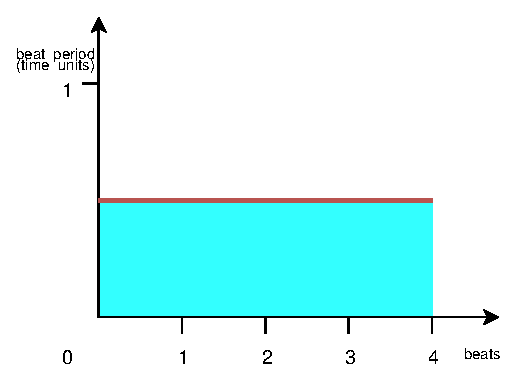
\includegraphics[width=1.4in]{eps/constant-bpm}
	\subfloat(b) \includegraphics[width=1.4in]{eps/step-bpm}
	\subfloat(c) 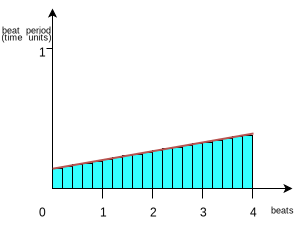
\includegraphics[width=1.4in]{eps/aprox-bpm}
	\subfloat(d) \includegraphics[width=1.4in]{eps/linear-bpm}
	\caption{Examples of tempo functions, between beats 0 and 4. In (a), we have a constant tempo of 120 bpm \textit{(bP = 0.5\,secs)}. In (b), there is a sudden (step tempo function) change, at beat 2, from 120 to 110 bpm \textit{(bP = 0.(54)\,secs)}. In (c), there is a sequence of step tempo change that are used to approximate a linear tempo change as seen in (d). In these examples, we chose to use beat period instead of BPM, for the y-axis, to make the section 2 explanation, regarding b(t) and t(b), more intuitive. } 
	\label{fig:tempochanges} 
\end{figure*} 

In \cite{wheresthebeat}, the authors used $T(t)$ instead of $T(b)$, resulting in a different integral and inverse of the integral for the tempo function. Despite the differences, the time map will produce the same results.

According to the previous definitions, a time map can be defined by $T(b)$, $bP(b)$, $t(b)$ and $b(t)$. For the current implementation, we provide three default for time mapping and tempo functions: linear, exponential and step tempo functions, all of them inspired in AudioParam automation functions.


\subsection{Supported Functions} 

In the following three subsections, we present the three forms for time maps included in our implementation: step, linear and exponential forms. All three share a set of terms related to tempo and time:
\begin{itemize}
	\item $b_0$, $b_1$: the initial and final score times;
	\item $T_0$, $T_1$: the initial and final tempos;
	\item $bP_0$, $bP_1$: the initial and final beat periods;
	\item $t$, $b$: the target time for tempo search and time mappings, $t$ for real time and $b$ for score time;
	\item $t_s$: the time offset, measured in seconds, for the function.
\end{itemize}

For each subsection, we define the generic functions and how are they mapped to a closed form.

\subsubsection{Linear}

Based on the definition of the formula used in AudioParam \textit{linearRampToValueAtTime} method
\begin{equation}
lin_{X_0,X_1,Y_0,Y_1}(x) = Y_0 + \Delta \cdot (x - X_0)
\end{equation}
with $\Delta = \frac{Y_1-Y_0}{X_1-X_0}$ defining the slope of $lin$. This function is not defined for $X_0=X_1$. Using this function, the tempo and beat period functions can be defined as
\begin{displaymath}
T(b)=lin_{b_0,b_1,T_0,T_1}(b),\,\,bP(b)=lin_{b_0,b_1,T_0,T_1}(b)
\end{displaymath}
where both functions are not defined for $b_0=b_1$. This "corner case" occurs when there is a sudden jump in tempo values. In that case, one should model the tempo change with a step tempo function. To obtain the mappings, we integrated the linear function and then obtained the inverse of the integral
\begin{equation}
\begin{split}
	 L_{X_0,X_1,Y_0,Y_1,C}(x) &=\int_{0}^{x} lin_{X_0,X_1,Y_0,Y_1}(x)\,d_x =\\
	&= \frac{\Delta}{2} \cdot (x-X_0)^{2} + Y_0 \cdot (x-X_0) + C
\end{split}
\end{equation}

\begin{equation}
L_{X_0,X_1,Y_0,Y_1,C}^{-1}(y) = \left\{\begin{array}{lll}
	sol_{1}(y) + X_0, & if\,\,sol_{1}(y)>0\\
	sol_{2}(y) + X_0, & otherwise
            \end{array}\right.
\end{equation}

\begin{displaymath} 
sol_{1}(y) = \frac{- Y_0 + k_1}{2 \cdot \Delta} \,\, , sol_{2}(y) = \frac{- Y_0 - k_1}{2 \cdot \Delta}
\end{displaymath}

\begin{displaymath} k_1 = Y_{0}^2 - \frac{4}{2} \cdot \Delta \cdot (C - y) \end{displaymath}

According to equations 5 and 6, the time mappings  are defined as
\begin{displaymath}
t(b) = L_{b_0,b_1,bP_0,bP_1,t_s}(b),\,\,b(t) = L_{b_0,b_1,bP_0,bP_1,t_s}^{-1}(t)
\end{displaymath}



\subsubsection{Exponential}

Consider the exponential function defined in \cite{wheresthebeat} as

\begin{equation}
exp_{X_0,X_1,Y_0,Y_1}(x) = Y_0 \cdot e^{k_2 \cdot (x - X_1)},\,\,k_2 =\frac{ \log{\frac{Y_1}{Y_0}}}{X_1 - X_0}
\end{equation}

and the tempo and beat period functions defined as 

\begin{displaymath}
T(b)=exp_{b_0,b_1,T_0,T_1}(b),\,\,bP(b)=exp_{b_0,b_1,T_0,T_1}(b)
\end{displaymath}

where all functions are not defined for $b_0=b_1$ (the same "corner case" as in the linear case). The time mappings for the exponential function can be obtained in a similar fashion:

\begin{equation}
\begin{split}
	E_{X_0,X_1,Y_0,Y_1,C}(x) &=\int_{0}^{x} exp_{X_0,X_1,Y_0,Y_1}(x)\,d_x = \\
	&= Y_0 \cdot \frac{e^{k_3 \cdot (x-X_0)} - 1}{k_3} +C
\end{split}
\end{equation}

and the inverse of the integral
\begin{equation}
E_{X_0,X_1,Y_0,Y_1,C}^{-1}(y) = \frac{\log{\frac{C \cdot (y - C) + 1}{Y_0}}}{k_3} + X_0
\end{equation}

and the final map between the generic functions and the time mapping functions is

\begin{displaymath}
t(b) = E_{b_0,b_1,bP_0,bP_1,t_s}(b),\,\,b(t) = E_{b_0,b_1,bP_0,bP_1,t_s}^{-1}(t)
\end{displaymath}

\subsubsection{Step}

The step function uses a similar tempo function to the AudioParam \textit{setValueAtTime},

\begin{equation}
step_{X_0,X_1,Y_0,Y_1}(x) = \left\{\begin{array}{lll}
	Y_{0}, & if\,\,x<X_1\\
	Y_{1}, & otherwise
            \end{array}\right.
\end{equation}

with the difference that the value jumps to $Y_1$ only for $x=X_1$ instead of $x=X_0$, like \textit{setValueAtTime} formula. The integral and inverse of the integral are defined as 

\begin{equation}
S_{X_0,X_1,Y_0,Y_1,C}(x) = \left\{\begin{array}{lll}
	Y_0 \cdot x + C, & if\,\,x<X_1\\
	Y_1 \cdot x + C, & otherwise
            \end{array}\right.
\end{equation}

\begin{equation}
S_{X_0,X_1,Y_0,Y_1,C}^{-1}(y) = \left\{\begin{array}{lll}
	\frac{y - C}{Y_0}, & if\,\,y<Y_1\\
	\frac{y - C}{Y_1}, & otherwise
            \end{array}\right.
\end{equation}

Again, the inverse of the integral is not defined for $Y_0 = 0 \lor Y_1 = 0$.  According to the previous formulas, we define the tempo and beat period functions as

\begin{displaymath}
T(b)=step_{b_0,b_1,T_0,T_1}(b),\,\,bP(b)=step_{b_0,b_1,T_0,T_1}(b)
\end{displaymath}

and the time mappings as 

\begin{displaymath}
t(b) = S_{b_0,b_1,bP_0,bP_1,t_s}(b),\,\,b(t) = S_{b_0,b_1,bP_0,bP_1,t_s}^{-1}(t)
\end{displaymath}

with $b(t)$ not defined for $T_0 = 0 \lor T_1 = 0$. This "corner case" is only problematic when modelling, with the step closed form, a full stop in the score/performance time.




\subsection{Beats Per Minute definition}


$T$ is (usually\footnote{In many DAWs like Ableton Live, Logic Pro Tools, Reaper, Ardour and LMMS, music tempo is expressed in Beats Per Minute (BPM). Still, it should be noted that music tempo can be expressed using, for example, italian tempo markings like \textit{Largo}, \textit{Adagietto}, \textit{Andante moderato} and so on.}) expressed in BPM. For example, $120\,bpm = \frac{120\,beats}{1\,min}$. But, usually, BPM is defined as 

\begin{equation}
BPM = \frac{60\,(secs)}{bP}
\end{equation}

with beat period measured in seconds. How do we deduce equation 5 from equation 1? If music tempo $T$ is measured as BPM, then $t=1 min$ and we can deduce from equation 1 that $ BPM = \frac{b}{1} = b$. Due to the fact that $1\,min=60\,secs$, we can make the following deduction:\\\\
$ T = \frac{b}{t} \Leftrightarrow \frac{1}{T} = bP = \frac{t}{b} $\\
$For\,\,\,t = 1\,min \Rightarrow T = \frac{b}{1} = b = BPM$\\
$For\,\,\,t = 60\,secs \Rightarrow bP = \frac{60\,(secs)}{BPM} \Leftrightarrow BPM = \frac{60\,(secs)}{bP}$\\

Throughout the remainder of this paper, unless stated otherwise, $T$ is measured as BPM and $t$ as seconds. Additionally, we use equation 16 to relate BPM and beat period instead of using the generic tempo/time relations stated in equations 1 to 4.



\section{Implementation}

In this section, we describe our JavaScript implementation for time maps, as defined in section 3. The current implementation has seven main features: 
\begin{itemize}
	\item find tempo $T$ at beat $b$, e.g.: what is the BPM $T$, at beat $b$;
	\item find tempo  $T$ at time $t$, e.g.: what is the BPM $T$, at $t$ seconds;
	\item find what is the beat $b$ at time $t$, e.g.: mapping time to beats;
	\item find what how much time $t$ has passed at beat $b$,e.g.: mapping beats to time;
	\item add, edit and remove tempo markers;
	\item add new closed forms for tempo functions;
	\item observe changes in a BPMTimeline instance through event listeners.
\end{itemize}

The first four features are related to tempo search and time mapping. The following two are related to tempo markers management. The final one offers a way to notify JavaScript components of changes in a BPMTimeline. A tempo marker is a JSON object that encodes the necessary information to evaluate local and global tempo functions: 
\begin{itemize}
 	\item \textit{endBeat}: beat $b_1$, stated by the developer when inserting the tempo marker in the BPMTimeline instance;
 	\item \textit{endTime}: time $t_1$, measured in seconds, calculated using $t(b_1)$ when inserting the tempo marker in the BPMTimeline instance; 
 	\item \textit{endTempo}: final tempo $T_1$, stated by the developer when inserting the tempo marker in the BPMTimeline instance;
 	\item \textit{endPeriod}: duration of a beat at the "end" of the corresponding tempo marker/function, measured in seconds, and calculated when inserting the tempo marker in the BPMTimeline instance;
 	\item \textit{type}: String identifying which closed form (step, linear, exponential or custom) is used to define the tempo and mapping functions, stated by the developer when inserting the tempo marker in the BPMTimeline instance.
\end{itemize}

The global tempo function, $T_{g}(b)$, is a non-continuous function, defined as 

\begin{displaymath}
T_{g}(b) = \left\{\begin{array}{lll}
	T_{l_1}(b), & if\,\,b_0 \leq b \leq b_1\\
	T_{l_2}(b), & if\,\,b_1 < b \leq b_2\\
	...\\
	T_{l_N}(b), & if\,\,b_{N-1} < b 
            \end{array}\right.
\end{displaymath}

where $T_{l_i}(b)$, $i=1..N$, are (local) tempo functions. A global tempo function is represented as a sorted array of tempo markers, sorted by \textit{endBeat}. Each BPMTimeline instance has only one global tempo function. Each tempo marker represents a local tempo function. The values $T_0$, $t_0$, $b_0$ and $t_s$ for each tempo are obtained by accessing the \textit{endTempo} (for $T_0$), \textit{endTime} (for $T_0$) and \textit{endBeat} of the previous marker in the global tempo function array.

As stated in section 1, (temporal) performance is a very important requirement. To fulfil this requirement, some trade-offs are needed for the different features available. As such, we make the following assumptions: 
\begin{itemize}
	\item in DAWs and DJ software, time maps are not changed very frequently during a live performance;
	\item as such, tempo search and time mapping are more important than tempo markers management.
\end{itemize}

We should note that the formulation, in section 2, for the tempo function $T(b)$ only mentions $b$. But, in practise, we could replace, in equations 8, 11, and 14 the terms $b_0$, $b_1$, $bP_0$, $bP_1$ and $b$ for $t_0$, $t_1$, $T_0$, $T_1$ and $t$, the tempo would will be the same for both cases ($T(b) = T(t)$).	

\subsection{Insertion, Edition and Removal of Tempo Markers}

There are three methods for tempo markers management: 
\begin{itemize}
	\item \textit{add\_tempo\_marker(String type, Number $b_1$, Number $T_1$)}: performs a binary search in the tempo marker array to find the neighbour tempo markers A and B, where $A.endBeat < b_1 < B.endBeat$. After finding those neighbours, insert the new tempo marker between them and update the \textit{endTime} field of all markers for which $\forall_{M} A.endBeat \geq M.endBeat$. If the new marker is the last one, only its \textit{endTime} field will be updated. If there is already a tempo marker with the same value for \textit{endBeat}, an exception will be thrown.
	\item \textit{remove\_tempo\_marker(Number $b_1$)}: performs a binary search in the tempo marker array to find the tempo marker A for which $M.endBeat=endBeat$. After that, removes M from the tempo markers array and update the \textit{endTime} field for all tempo markers $M$ that $\forall_{M} A.endBeat \geq M.endBeat$. If there is no tempo marker A for which $M.endBeat=endBeat$, then an exception will be thrown.
	\item \textit{change\_tempo\_marker(Number $b_1$, Number $b_{1}'$, Number $T_{1}'$, String newType)}: removes the tempo marker from the array and adds the new version. If there is no tempo marker A for which $M.endBeat=b_1$, then an exception will be thrown.
\end{itemize}

\begin{figure*}
	\centering
	%COLOCAR A IMAGEM demo.png [width=7in]
	\includegraphics[width=6in]{demo.png}
	\caption{A simple demo page with a graph plotting the output of BPMTimeline.tempo\_at\_beat, and a table listing the markers of the BPMTimeline instance.}
	\label{fig:demosurface} 
\end{figure*}

These four methods for tempo marker management have the temporal complexity is $O(N)$. This is due to the usage of a binary search over a sorted array, $O(log_2 N)$, and the calculation for the \textit{endTime} field, $O(N)$. As such, we have $O(log_2 N) + O(N) = O(N)$.

To add a new closed form for tempo functions, the developer can use the \textit{add\_tempo\_marker\_type(String type, Function tempoFn, Function integralFn, Function inverseIntegralFn)} method. Parameters 2, 3 and 4 are explained in section 2 and their API must be defined as: 
\begin{itemize}
	\item \textit{tempoFn(Number $b_0$, Number $b_1$, Number $T_0$, Number $T_1$, Number $b$)}: implementation of the tempo function $T(b)$, as defined in section 2;
	\item \textit{integralFn(Number $b_0$, Number $b_1$, Number $T_0$, Number $T_1$, Number $t_s$, Number $t$)}: implementation of the mapping $t(b)$, as defined in section 2;
	\item \textit{inverseIntegralFn(Number $b_0$, Number $b_1$, Number $bP_0$, Number $bP_1$, Number $t_s$, Number $b$)}: implementation of the mapping $b(t)$, as defined in section 2.
\end{itemize}

This method has temporal complexity of $O(1)$ (on average) because it only performs an insertion in an associative array.

\subsection{Tempo Search and Time Mapping Methods}

The current implementation has 4 methods for this task:

\begin{itemize}
	\item \textit{beat(Number t)}: Maps real time $t$ to score time, $b(t)$. First, performs a binary search over the tempo markers array to find tempo markers A and B for which $A.endTime < t < B.endTime$. If the search returns both A and B, perform the mapping $b(t)$ using \textit{inverseIntegralFn( A.endBeat, B.endBeat, A.endPeriod, B.endPeriod, B.endTime, t )}. If the search returns just a marker, then then $b(t) = A.endBeat$.
	\item \textit{time(Number b)}: Maps score time $b$ to real time, $t(b)$. First, performs a binary search over the tempo markers array to find tempo markers A and B for which $A.endBeat < b < B.endBeat$. If the search returns both A and B, perform the mapping $b(t)$ using \textit{integralFn( A.endBeat, B.endBeat, A.endPeriod, \\B.endPeriod, B.endTime, b )}. If the search returns just a marker, then then $t(b) = A.endTime$.
	\item \textit{tempo\_at\_time(Number t)}: Returns tempo at real time $t$. First, performs a binary search over the tempo markers array to find tempo markers A and B for which $A.endTime < t < B.endTime$. If the search returns both A and B, obtain the tempo through \textit{tempoFn( A.endTime, B.endTime, A.endTempo, B.endTempo, t )}. If the search returns just a marker, then the tempo is equal to A.endTempo.
	\item \textit{tempo\_at\_beat(Number b)}: Returns tempo at score time $b$. First, performs a binary search over the tempo markers array to find tempo markers A and B for which $A.endBeat < b < B.endBeat$. If the search returns both A and B, obtain the tempo through \textit{tempoFn( A.endBeat, B.endBeat, A.endBeat, B.endBeat, b )}. If the search returns just a marker, then the tempo is equal to A.endTempo.
\end{itemize}

All four methods have temporal complexity of $O(log_2 N)$ due to the usage of binary search of a sorted array. If no marker is found in each of these four methods, an exception is thrown.

\subsection{Event Listeners}

Each BPMTimeline instance is observable: all changes (i.e. everytime a marker is added, edited or removed) in the instance results in an event being created and a set of event listeners will be invoked to deal with that event. In order to register/remove event listeners in a BPMTimeline instance, the class provides two functions:
\begin{itemize}
	\item \textit{add\_event\_listener(String observerId, String eventType, Function callback)}: register an event listener for events of the following types: \textit{"add-tempo-marker"}, \textit{"change-tempo-marker"} and \textit{"remove-tempo-marker"}.
	\item \textit{remove\_event\_listener(String observerId, String eventType)}: remove the listeners, that were registered by observerId, for events with eventType type.
\end{itemize}	

The \textit{observerId} argument is used to prevent conflicts between two observers using the same function as event listener. Each event object has the following schema:

\begin{lstlisting}
{ type: String, 
  oldMarker: MarkerDescription, 
  newMarker: MarkerDescription }
\end{lstlisting}

The \textit{type} field can have one of the following values: \textit{"add-tempo-marker"}, \textit{"remove-tempo-marker"} or \textit{"edit-tempo-marker"}. When \textit{type} is equal to \textit{"add-tempo-marker"}, the \textit{oldMarker} field does not exist. When \textit{type} is equal to \textit{"remove-tempo-marker"}, the \textit{newMarker} field does not exit. Each \textit{MarkerDescription} instance has the following schema: 
\begin{lstlisting}
{ startBeat: Number, endBeat: Number, 
  startTime: Number, endTime: Number, 
  startTempo: Number, endTempo: Number, 
  type: String }
\end{lstlisting}

\textit{startBeat} and \textit{endBeat} define where does the marker tempo functions start and end in score time and \textit{startTime}, \textit{endTime} state where does the marker tempo functions start and end in real time.

\section{Use Cases}

To date, we have explored three use case scenarios for BPMTimeline: (1) \textit{event scheduling}, mapping time values in AudioContext.currentTime in order to schedule oscillator plays; (2) \textit{auto-syncing} of several audio players to a dynamic master tempo, in a similar fashion to Ableton Live; (3) \textit{time rulers}, for real and score times, related through a BPMTimeline instance.

\subsection{Event Scheduling and Effect Automation}

BPMTimeline can be used to control, through the mapping $t(b)$, the scheduling of Web Audio API (WAA) Audio Nodes, like Audio Buffer Source Nodes and Oscillator Nodes), and their Audio Parameters. Assuming that for $beat=0 \Rightarrow AudioContext.currentTime=0$, the developer can play a buffer source node and/or an oscillator node using the following code:

\begin{lstlisting}
/** Initial tempo of 60 bpm. **/
var tl = new BPMTimeline(60);
var a_t_m = tl.add_tempo_marker;
a_t_m({type:"linear",endBeat:10,endTempo:200});
a_t_m({type:"linear",endBeat:15,endTempo:10});
a_t_m({type:"linear",endBeat:20,endTempo:400});
a_t_m({type:"linear",endBeat:60,endTempo:60});
var ctx = new AudioContext();
var osc = ctx.createOscillator();
/** Play 20 beats. **/
for (var i=0; i<20; i++) {
 scheduleNote(osc, 'G3', i, 0.5, ctx.currentTime);
}
osc.connect(ctx.destination); osc.start();
\end{lstlisting}

resulting in a half-beat pulse train, that increases and/or decreases its tempo throughout the time line. This code is available in our Git repository.\footnote{https://github.com/echo66/bpm-timeline.js/blob/master/demos/demo3.html} Additionally, this module could be used to control the tempo in libraries like Tuna.js\footnote{https://github.com/Theodeus/tuna} which, as far as we know, does not have any implementation for constant or dynamic tempo.

\subsection{Automatic Audio Player Synchronization}

Another use case is the synchronization of audio audio players to a master tempo time line, which is very common in live music performance applications like Ableton Live. In one of our prototypes, we share a BPMTimeline instance (the master tempo) with several audio players. The stretching factor for each player is determined through the relation between the master tempo and the tempo of the audio segment being played/stretched.\footnote{https://github.com/echo66/OLA-TS.js/blob/master/SegmentProcessorV3.js\#L121}

\subsection{Time Rulers}

WAVES UI library \cite{wavesui:wac2015} provides a set of music related UI components (automation lines/breakpoints, waveforms, time annotations, time rulers, etc) for HTML5. One of those components, time axis, allows developers to present two time rulers: one for real time (seconds) and another for score time (beats), both related through a constant tempo (BPM). In order to use BPMTimline with WAVES UI library, the developer must decide what will be "static" time line\footnote{If we choose beat time to become "static", the tempo changes affect the real time ruler.}, either real time or score time, in the rulers. Traditionally, DAWs make score time as the "static" time line. In order to do the same with WAVES UI, the developer will need to state the time values for segments, breakpoints, waveforms and traces in score time.

\section{Evaluation and Comparison}

In this section, we evaluate BPMTimeline and compare it with Tone.js, the most advanced JavaScript implementation for tempo manipulation.
\begin{itemize}
	\item \textbf{Time Maps}: Tone.js does not offer any time mapping feature.
	\item \textbf{Tempo Functions}: Tone.js and BPMTimeline offer a similar set of basic tempo functions: step, linear and exponential. Still, with Tone.js, it is possible to schedule an arbitrarily complex tempo function using \textit{setValueCurveAtTime} Tone.Signal method.
	\item \textbf{WAA}: Tone.js uses a Tone.Signal object for tempo automation, a class that uses a Gain Node to schedule changes for tempo, effect parameters, etc. BPMTimeline does not have any dependence on specific JavaScript environments besides a compliant ECMAScript 5 implementation.
	\item \textbf{NPM}: Tone.js has a NPM module available. Still, the current implementation does not allow to use Tone.js within node.js or io.js due to its dependence on WAA.
	\item \textbf{Time markers}: BPMTimeline requires the user/developer to schedule tempo changes using score time values. In Tone.js, due to its dependence on WAA, tempo changes are scheduled with performance time.
\end{itemize}

\section{Conclusions and Future Work}

BPMTimeline provides an intuitive API for developers to relate time and beats, according to a custom tempo function. Due to the search method employed, we expect to minimize the (temporal) performance impact of time mapping and tempo search functions.

The next step will be the support for arbitrarily complex functions. Instead of specifying the closed form for all tempo functions ( there are infinite tempo functions), one could sample an tempo function and interpolate the resulting sequence with a set of linear tempo functions.

After that, we plan to integrate BPMTimeline in browser live coding environments like Flocking \cite{flocking:icmc2014}, Tone.js \cite{tonejs:wac2015} and UI libraries/frameworks like WAVES UI \cite{wavesui:wac2015}. 

%ACKNOWLEDGMENTS are optional
%\section{Acknowledgments}
%This work was partly supported by national funds through FCT – Fundação  para a Ciência e Tecnologia, under project EXCL/EEI-ESS/0257/2012.
%This work was supported by national funds through Fundação para a Ciência e a Tecnologia (FCT) with reference UID/CEC/50021/2013.

%
% The following two commands are all you need in the
% initial runs of your .tex file to
% produce the bibliography for the citations in your paper.
\bibliographystyle{abbrv}
\bibliography{sigproc}  % sigproc.bib is the name of the Bibliography in this case
% You must have a proper ".bib" file
%  and remember to run:
% latex bibtex latex latex
% to resolve all references
%
% ACM needs 'a single self-contained file'!
%
\balance
\end{document}
